% Created 2019-04-13 Sat 22:52
% Intended LaTeX compiler: pdflatex
\documentclass[12pt,a4paper,man]{report}
\usepackage[utf8]{inputenc}
\usepackage[T1]{fontenc}
\usepackage{graphicx}
\usepackage{grffile}
\usepackage{longtable}
\usepackage{wrapfig}
\usepackage{rotating}
\usepackage[normalem]{ulem}
\usepackage{amsmath}
\usepackage{textcomp}
\usepackage{amssymb}
\usepackage{capt-of}
\usepackage{hyperref}
\renewcommand{\baselinestretch}{1.5}
\usepackage{apacite} \usepackage{algorithm} \usepackage{listings} \usepackage[noend]{algpseudocode}  \usepackage{indentfirst}  \usepackage{fancyhdr} \usepackage{stringstrings}
\usepackage{geometry} \geometry{ a4paper,  total={170mm,257mm}, left=20mm, top=1in, foot=0.3in}
\usepackage[final]{pdfpages}
\usepackage{placeins}
\usepackage{cmap} \usepackage[T1]{fontenc}
\usepackage[raggedright]{titlesec}
\author{Ibrahim}
\date{\today}
\title{Final Report I: Affective Movie Evaluator}
\hypersetup{
 pdfauthor={Ibrahim},
 pdftitle={Final Report I: Affective Movie Evaluator},
 pdfkeywords={},
 pdfsubject={},
 pdfcreator={Emacs 26.1 (Org mode 9.1.9)}, 
 pdflang={English}}
\begin{document}

%set the first page
\setboolean{@twoside}{false}
\begin{titlepage}

\includepdf[pages=-,pagecommand={},width=\textwidth]{FirstPage.pdf}
\end{titlepage}
\maketitle
\tableofcontents

%FIX ISSUE WITH CHAPTER TITLE MARGIN
\makeatletter
\def\ttl@mkchap@i#1#2#3#4#5#6#7{%
  \ttl@assign\@tempskipa#3\relax\beforetitleunit
  %\vspace*{\@tempskipa}% NEW
  \global\@afterindenttrue
  \ifcase#5 \global\@afterindentfalse\fi
  \ttl@assign\@tempskipb#4\relax\aftertitleunit
  \ttl@topmode{\@tempskipb}{%
    \ttl@select{#6}{#1}{#2}{#7}}%
  \ttl@finmarks  % Outside the box!
  \@ifundefined{ttlp@#6}{}{\ttlp@write{#6}}}
\makeatother 

%CHAPTER TITLE STYLE
\titleformat{\chapter}[hang] 
  {\normalfont\huge\bfseries}
  {\chaptertitlename{ \thechapter : } }
 {0in}
  {} 



\newpage
\begin{abstract}
	Write Abstract here.  

\end{abstract}

\newpage
\topskip0pt
\vspace*{\fill}
\section*{Declarations}
I hereby declare that the report presented here as part of the requirement of BIT304 is original and no parts of this report had been plagiarised from any other resources unless those indicated with proper referencing.  This report will be the property of HELP University and cannot be distributed in any form without the written consent of HELP University.
\\\\Student Names:
\begin{description}
 \item Mohamed Shaatha Ibrahim (B1301746)
 \item Elebe Faith Alfred (B1301511)
\end{description}
Date: 12-04-2019
\vspace*{\fill}

\renewcommand{\abstractname}{Acknowledgement}
\begin{abstract}
	Aknowledgements here.
\end{abstract}



%set the header
\newcommand\SentenceCase[1]{
  \caselower[e]{#1}
  \capitalize[q]{\thestring}
}
\newcommand*\parttitle{}
\let\origpart\part
\renewcommand*{\part}[2][]{%
   \ifx\\#1\\% optional argument not present?
      \origpart{#2}%
      \renewcommand*\parttitle{#2}%
   \else
      \origpart[#1]{#2}%
      \renewcommand*\parttitle{#1}%
   \fi
}

\pagestyle{fancy}
\fancyhf{}
\rhead{\thepage}
\lhead{\parttitle{}: \leftmark}
\cfoot{\thepage}
\renewcommand{\chaptermark}[1]{\markboth{#1}{}}


\part{Proposal}
\label{sec:orged29340}
\chapter{Introduction}
\label{sec:orgeae5cb7}

Movie production studios use test screening in order to determine whether their movies will succeed. Recently, internet movie distributors such as Netflix and Amazon have started taking more control of the production of their content, it is more beneficial for studios to re-edit their movie once they can predict that the product is going to fail. While there are automated sentiment analysis tools used to measure how well the audience reacts to test screening, most of the feedback is still taken from questionnaires and the audiences subjective evaluation.

We aim to provide an automated, movie evaluation system which is going to analyse the audience watching the movie and predict an overall score. Our system is intended to supplement the existing manual process of test screenings. We are not proposing a system to replace the existing subjective evaluations given by the audience.

The aim of this project is to develop a system that can evaluate how good a movie is, by analysing both face and body postures of the audience. In order for this to work we provide the system a video file consisting of audience reactions, and the system will tell us how good a movie is within a rating metrics, we will define later. It is important for us to state, that we are not proposing a real-time system here; the system accepts a recording of the raw data - which is currently defined as video file, and can be any other form of measurement - as the primary input.

A system like this can aid us develop further, a more general system that can evaluate how good a certain product or presentation is by analysing the audience reaction limited by a certain context. In our case the product is a movie, and how the audience reacts may depend on what genre of movie they are watching, or what kind of experience they were expecting beforehand. It is likely that our system may not work well without knowing these information. Systems like these are also related to computer vision with Emotion AI technologies, such as face based lie detectors, which uses the same techniques to work.

\chapter{Background}
\label{sec:orgb6eafb2}
For a long time movie industry have used statistical modeling and machine learning to predict, the success of movies based on high level data. While there have been several works in early to mid 2000’s, which takes in multimedia information to form a representation for the user’s emotions (Zhang, S.,  2008; Wu T.L, 2008), the earliest work we could find that specifically focus on movie scenes was by Soleyman et. al.

Quite recently, there have been interest in using deep learning techniques to analyse audiences facial data such as (Saha, S. et al., 2018), to predict whether an audience enjoyed the movie, most notably research work that has been funded by The Walt Disney Company (Deng, Z. et al, 2017). The purpose of their research is to use facial emotion recognition techniques, to analyse the emotion of the audience in order to improve the movies.

Research has shown that over 90\% of our communication can be non – verbal (Algorithmia, 2018). Non- verbal communication which includes facial expressions and body postures among others can be used to determine the emotional state of a human being. According to Paul Ekman (Ekman P, 1992), there are basically six types of human emotions namely:  happiness, sadness, disgust, fear, surprise, and anger. 

The system we are proposing is going to take in a video file of an audience reacting to a movie and attempts to determine whether the audience liked that movie. It will use emotion recognition and body pose to quantify the overall reaction in order to determine whether the viewer enjoyed the movie or not. 

Although, idea of such a system is not new, we have not been able to find an existing system that considers both body pose and facial emotion data to create a model that can predict. Previous work such as (V Ramanarayanan et al., 2015), which evaluates a presenter by using a very similar technique that we are planning, performed very poorly compared to the human judges. However, we are a bit more optimistic, since movies are designed to elicit certain emotional responses and audiences in average exhibit similar reactions. Such a system, maybe useful in the film industry to analyse the reactions of the test audience as a supplement to the usual questionnaires. 
The problem we are trying to solve is that film studios screens movies to test audience, and audience writes back a subjective feedback usually on paper. Our software is intended to complement the existing evaluation procedure, by providing an automated evaluation of audience's experience that is less subjective and provide a numerical score that represents audience's sentiment more accurately.

Affective Analysis is already used by marketing giants such as Coca-Cola to predict the effectiveness of their advertisement on target test audiences. Affective movie analysis could prove to be valuable to streaming services that distributes their own content and have more control over the productions such as NetFlix.

\chapter{Issues}
\label{sec:org25b9773}
Our system is not real-time but still requires heavy computing power in order to run. This means the admin will often have to run multiple processes for analysis and come back later for the result. Our system does not support multiple processes yet, while it is possible for our system to run a process on a remote server or a cloud computer service via ssh and http, the admin still have to wait for the analysis to be completed. 

In order to minimize the scale of the problem, the first few iterations of the problem deals with only a single audience member. The largest audience we will be designing our system will be for a group of two to four person, under controlled lighting environment. Unless we have access to infrared cameras and better computing facilites, we will not be able to overcome these limitations. 

Our video can only have one person in front of the camera. The application is not able to give proper result if there are faces in the background when the audience member is reacting. Presence of another person in the room currently effects the resulting data, and it is very time consuming for a human to verify whether the recorded data does not have any background face. However, as we wrote our detection algorithm to choose the largest region of interest in the image, the fail cases we have observed usually consists of background posters and wallpapers with larger face than our subject.

One of the weakness we have is in the accuracy of the face detection algorithm. OpenCV's default facial detection algorithm, (Viola-Jones full frontal model) requires the audience member to face the camera directly. However, we plan to implement a more accurate face detection algorithm at the risk of increasing computing time.

Right now our system uses an externel media player known as VLC media player, to play the movie while being recorded in use case 1. The system admin is usually required to install the software manually. However on Windows based systems, it is sometimes not possible to find the 

\chapter{Benefits and Constraints}
\label{sec:org315254b}
For our current iteration the system can analyse only one audience member. The reason for this limitation is that we initially wanted to start the project with a smaller scope and also to reduce the amount of tasks we might have for the first iteration. Even in our future iterations, we will not be analysing and audience consisting of more than a handful of person, unless we get better camera equipments.

Another issue faced by us is that facial emotion recogntion is not working that well, for now. In order to improve the accuracy of the FER model we plan to write separate test cases.

Since our system takes a long time to analyse, we had to modify our "Analyse Video" use case into two seperate parts. Instead of directly providing a video file to run analysis and immediately getting the results and visualisations, our system actually requires the admin to run two seperate instance of analysis, facial emotion analysis (FER) and pose analysis (BEGR). Running an instance of analysis will produce the required data file, which can then be visualised as a time-series and processed to be sent for our movie evaluation ML model.


\chapter{Project Description}
\label{sec:org51f87c8}

Our system analyses audience reaction, and attempt to predict a score.

\chapter{Project Aims and Objectives}
\label{sec:orge95c394}
The aim of our project is to develop a system that can evaluate how good a movie is, by analysing both face and body postures of the audience. In order for this to work we provide the system a video file consisting of audience reactions, and the system will tell us how good a movie is within a rating metrics, we will define later. It is important for us to state, that we are not proposing a real-time system here; the system accepts a recording of the raw data - which is currently defined as video file, and can be any other form of measurement - as the primary input.
\begin{itemize}
\item system like this is very useful for movie studios, which often relies on test audience in order to predict whether their movies are going to be successful and a system like this can aid in measuring the audience reaction more accurately.
\end{itemize}
The objectives we have set for our project are the following:
Define the metrics by which the system is going to give the score before we create the evaluation model. (e.g: value between 0.0-1.0 or a discrete grading system, like A+, A,  
\begin{itemize}
\item Research the requirements of the dataset, and methodologies before week 3.
\item Find or create the required test datasets for in order to complete objective 6.
\begin{itemize}
\item Dataset for the emotion recognition subsystem
\item Dataset for body pose subsystem.
\item Dataset for the whole system: Video recordings of audiences reacting to movies.
\item Determine accuracy of the overall project by comparing its output to existing scoring systems.
\end{itemize}
\item To prove that we are using state of the art technologies in our system; produce:
\begin{itemize}
\item Accuracy report for Emotion recognition
\item Accuracy report Body pose/action estimation
\end{itemize}
\end{itemize}

\chapter{Project Scope}
\label{sec:orgadfe16e}
\begin{itemize}
\item For developement purpose, we will be dealing with short movies mostly.
\item We will be recording atleast 12 subjects, watching multiple movies.
\end{itemize}

\chapter{Software and Hardware Requirements}
\label{sec:org4b3864a}

\section{FUNDING SOURCES}
\label{sec:orgf7a8dd4}
As mentioned before we do not have any corporate and industry backing, therefore we are expecting HELP School of ICT to provide any possible funding we may require, if requested. Since the University already have most of the assets we require for our FYP1, we will require permission from the IT department to use the facilities, for our project.
As for FYP2, the tools and resources we require for data collection and obtaining ground truth can only be determined after we complete the first part of our project.

\section{Minimum hardware requirements}
\label{sec:org9e0effb}
Although, our system can run with a laptop with a webcam we designed the system with the following requirements in mind.

\begin{table}[htbp]
\caption{\label{table:mreq}
Minimum Hardware Requirements}
\centering
\begin{tabular}{|l|l|l|l|lp{3cm}|}
\hline
No & Item & Usage & Qty\\
\hline
1 & VGA USB Camera & Used to record audience & 1\\
2 & Computer Terminal & Our application need to run & 1\\
 & (Desktop/Laptop & on an computer with a & \\
 & /SmallFactor) & display terminal. & \\
\hline
\end{tabular}
\end{table}

\section{Recommended hardware requirements}
\label{sec:orgd32423a}

\begin{table}[htbp]
\caption{\label{table:mxreq}
Recommended Hardware Requirements}
\centering
\begin{tabular}{|l|l|l|l|lp{3cm}|}
\hline
No & Item & Usage & Qty\\
\hline
1 & HD Camera & Used to record audience & 1\\
2 & High-end Desktop Computer & Our application need to run & 1\\
 &  & on an computer with a & \\
 &  & display terminal. & \\
3 & CUDA compatible Graphics & Used to improve video & 1\\
 & Card - NVDIA geforce & analysis models & \\
 & gtx 1080 ti &  & \\
\hline
\end{tabular}
\end{table}

\chapter{Developement Methodology}
\label{sec:orga1a07bd}
To give you the context of the reasoning behind our decision, we would like to discuss a brief overview of commonly used development methodologies first. The most commonly followed methodologies for data-science projects are either SEMMA or CRISP-DR methodologies. SEMMA is a methodology developed by SAS institute, while CRISPR-DR method was originally developed in a joint effort by five companies, and further improved by data mining industry, most notably by IBM. 

The main difference between both methodologies are that CRISPR-DR considers business understanding of the process and also considers model deployment and the results. SEMMA is mainly used for data mining projects, which does not consider business aspect. The methodology we chose for our project is SEMMA methodology.

The reason we chose SEMMA is that, we wanted to keep option generalise our problem scope later, for example we wanted to apply what the system does in other scenarios than movies. Also, business project timelines and research project timelines are usually incompatible, and this is a fact we need to consider while planning early on, since machine learning projects falls under the latter. So not considering the business aspects of the project, will be an advantage for us given the time we  have. 

SEMMA methodology consists of 5 phases (Sample, Explore, Modify, Model and Assess). SEMMA methodology gives us freedom to reiterate from any step, as we require. It does not have a definitive cycle for iteration, which makes it a more simple and less rigid framework to follow, compared to CRISP-DR (Palacios, 2017). 
Sample:  First step of of SEMMA involves collecting all data samples.
Explore: Understand the problem through exploration of sample data. Exploration can be helped through visualisations and other data analytic tools.
Modify: Next steps, involves selecting which variables/features can be used, how they can be transformed or processed in order to create a model.
Model phase consists of selecting and creating a model
Assess: Finally we evaluate how well the model performed, and determine whether it is useful in real world situation.
In order to properly use SEMMA methodology into our project we are going to we are going to collectively apply the methodology to three separate components of our system that we have previously identified; the facial emotion subsystem, body emotion subsystem and movie evaluation model. After we started planning, we realized given only two team members, it was actually impossible for us to go through the whole system with one iteration within one semester. 

Therefore, we have split the project into two phases. Each phase is considered iteration by itself, because during the first phase, we build the first two components of our pipeline simultaneously (by two members), such that they both go through the SEMMA process at the same time. During the process, we also ensure both components are integrated before we start the next phase.

Then, we will start next iteration; go back to the sample stage to work on the final part of our project. For example, after the Assess phase of the emotion models we will be starting again from Sample phase again, and ensure everything in the pipeline is working well. This does not mean we define the term “phase”  and “iteration” as being interchangeable. 

Eventually, given the results it is possible we may plan a new iteration, if necessary. For example, if after assessing the Movie Evaluation Model, it performed poorly, we may go back to either Modify stage to pick better features to be passed into the model or we can even go back to Model stage to pick a different model.

The first planned iteration of  our project we will be focused on building the facial emotion and body pose emotion subsystem, which will be for simplicity hence referred to as “Emotion Model” and “Pose Model”, respectively. The second part of our project will be the combined system along with “Movie Evaluation Model”. Most of our work on Movie Evaluation Model, is currently planned to commence on the second part of our internship (FYP2), and the gantt chart we have proposed in the Appendix section might significantly change.

As our primary version control system we will be using gitlab as our github repository. Also, since SEMMA does not define a project management style, we will be using kanban/scrum like board feature on gitlab, to organize the tasks that we will be doing. However, we will not be adhering to any strict project management style, which is very prevalent in the software industry.

As for the specific techniques we will use throughout the development, our idea is to analyse existing literatures, and compare notes and follow general data mining/modeling techniques with fewer brainstorm sessions. In order to obtain the ground truth while collecting the data, our current idea is to use questionnaires after recording a subject’s reaction. Alternatively, it’s possible for us to measure blood pressure or any other means of observation if possible, and we will consider that for our FYP2.

\part{Project Management Plan}
\label{sec:org6072230}
\chapter{Introduction}
\label{sec:org7f9b046}

\chapter{Work Breakdown Structure}
\label{sec:orgae442cf}
\chapter{Risk Management}
\label{sec:org4c086f1}
\chapter{Gantt Chart}
\label{sec:org14a2ee9}
We created the work breakdown structure during our project plan, and we grouped each task under a phase in our methodology.
Then we estimated time for each task and prioritsed them, finally creating a project timeline (Gantt CHart)

\part{Requirement Analysis}
\label{sec:org8f7abab}
\chapter{Introduction}
\label{sec:org540b329}
Since the conception of the project plan, our initial goal for the first iteration was to create a system that is going to analyse the facial emotion and body posture emotion independently and construct a data representation such as a time-series from the analysis. We delegated the primary goal of our project, which is to use that data to train and create a model that can score movies for later iterations intentionally, so it will give us time to reconsider our methods and also create dataset in between the downtime.

Like any other software developement project, our approach was to first of all analyse the system and identify. Practically, most of the requirement analysis was done while we were creating the project plan, while we did not thoroughly document it in the proposal itself. This part of the document was later updated to reflect the change in number of use-cases in our iteration 1, after we realised that we are not able to fit the three initial use-cases we planned into the first iteration.

Along with the project's functional requirements and non-functional requirements, we will also try to give an overview of the requirements from the machine learning perspective. We will try to state the ML problem, and define the requirements and structure for the problem. It should be noted by now, our system will consist multiple ML algorithms interacting with each other and a portion of has to be designed by us. 

We also wanted to complete all the software design and engineering intensive tasks as early as possible so we can focus on the machine learning aspects of our project. Thus, a large portion of this iteration is writing the code for user interaction, and designing processes within the system that can perform independent of the type of user interface.

Initially, we like we planned we worked on the facial analysis, and posture analysis portion of the code seperately. Later on we refactored and integrated the code as seperate modules into a single codebase with the help of object-oriented programming.



\chapter{Requirement Summary}
\label{sec:org9315640}
The first thing we did during our first meeting was infact to identify all the stakeholders and actors who interacted with the system. While we discussed the naming conventions of the actors involved during the later meetings, it was early on established that only one user directly interacts with the system and can be considered to be the primary user.

Our systems consists of mainly this one user controlling the application directly. Ideally this user is a system operator, hired by the production company with a knowledgeable background in IT and system administration. Throughout this document we refer to this user, simply as \emph{Admin}. We should note that the user \emph{Admin} is not really a recognized object within the system and thus does not have a login function. \emph{Admin} refers to whoever is operating the system.

\section{Actors and Stakeholders}
\label{sec:org247cea3}
\begin{enumerate}
\item Admin
\label{sec:orgdc49e6c}
\item Subject
\label{sec:org84ffcdc}

An \emph{Admin} can use the system to record audiences watching a movie. Right now, in order to do that, the movie must exist within the computer system first. Admin is supposed to launch our application, and provide the details of the audience member and the movie, because the system does not yet store the metadata of the movies yet. The movie object is not considered as an object of the system in this iteration.

\begin{itemize}
\item Admin is able to Record a video of a \emph{Subject} watching a movie.
\item Admin is able to Analyse a video of a subject
\begin{itemize}
\item Produce time-series.
\end{itemize}
\end{itemize}

While the UML for iteration 1 might not directly hint that subject is indeed a part of the system, it is going to be added as an Object in our future iteration. We did not include the \emph{Subject} as an object that is in the system, yet.
\end{enumerate}


\section{Object represented in the system}
\label{sec:orgfaf2ce2}
\begin{itemize}
\item Movies
\item Samples
\end{itemize}

\section{Hardware Architecture / Layout}
\label{sec:orgafdeda2}

\section{Pipeline diagram}
\label{sec:orgdbe8734}

\chapter{Functional Requirements}
\label{sec:orgeed3396}
\section{Use-Case Diagrams}
\label{sec:org5530707}
While designing of the use-cases we only thought from a logical/business perspective and not included the "technical" usecases, as our methodology and approach does not heavily rely on UML. 


\begin{center}
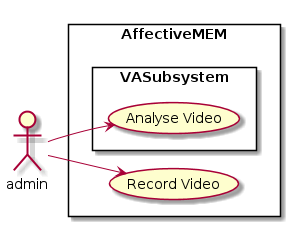
\includegraphics[width=.9\linewidth]{./img/auc.png}
\end{center}


In figure \ref{fig:auc}, you can see that the Analyse Video is bound within a subsystem of Affective Movie Evaluator. The reason

While there is a weak implementation of other use cases, the two use-cases shown in the diagram \ref{fig:auc}, are the main goal of our current iteration until now.

\begin{center}
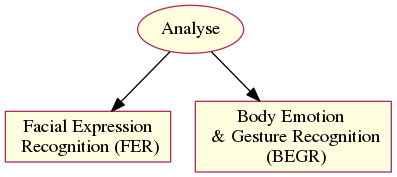
\includegraphics[width=.9\linewidth]{./img/auc_exp.png}
\end{center}


It would have been ideal for the sake of this documentation for Analyse use case to include two "technical" use-cases, "Analyse FER" and "Analyse BEGR", so that it is easier to credit the two team members, but it would not have been accurate. Ideally a use case should show an added value to a system, and seperating them does not really contribute the value to from either logical or design perspective. 


\begin{table}[htbp]
\caption{\label{table:auc1}
Analysis usecases}
\centering
\begin{tabular}{|l|l|lp{3cm}|}
\hline
\textbf{Use Case 1} & Record Video\\
\hline
Goal in Context & To record an audience member's video and store it.\\
\hline
Primary Actors & - Admin\\
Secondary Actor & - Audience\\
\hline
Description & Use camera to record and store video session of an audience\\
 & watching a movie screening.\\
\hline
\hline
\textbf{Use Case 2} & Analyse Video\\
\hline
Goal in Context & To extract an audience's facial and body pose data from a\\
 & video file and store it as readable data.\\
\hline
Primary Actors & - Admin\\
Secondary Actor & - Audience\\
\hline
Description & Use camera to record and store video session of an audience\\
 & watching a movie screening.\\
\hline
\end{tabular}
\end{table}



\section{High-Level Use Cases}
\label{sec:org33ba83f}
\chapter{Non-Functional Requirements}
\label{sec:org10552e8}
\section{Technical Requirements}
\label{sec:orgb3cc618}

\section{Usability Requirements}
\label{sec:org14185be}
\section{Reliability Requirements}
\label{sec:org96cd840}
\section{Security Requirements}
\label{sec:org30d67e6}


\part{Iterations}
\label{sec:org494f333}
\section{Introduction}
\label{sec:orgdfb864c}
Note, that we combined SEMMA phases with SDLC phases in our project timeline. The SEMMA phase are not analogous to an SDLC phase, and we've learned that there may exist no standard for such analogy. For example most software engineers and feature engineers tend to write code during the Sample phase while ML engineers may work on something else.

After our analysis phase we broke down the project into completable tasks. In-order to identify the completable tasks, we thought of the project in terms of user-story/use-case perspective and also by identifying the independent components of the system, from our analysis. We thought of the first input data that will pass through the pipeline, and how it will be processed along to get the results we wanted. For example, if our initial data is video files captured by a camera device, the system must have to at somepoint interact with a camera object, therefore it is very likely during our design phase that we may need to create a camera object for a module.


We only have one Iteration for this part of our final year project.
Initially the work was divided between the two part.
Use case one was primarily developed by Ibrahim and designed by Faith.

Use-case two's main two sub-components were developed and tested independently and later on we re-integrated our work into a single codebase.

\chapter{Iteration 1}
\label{sec:org3b1ef87}
\section{Introduction}
\label{sec:orgb06e01d}

\section{Purpose}
\label{sec:org707a3dd}
The purpose of this iteration is only to produce:
\begin{enumerate}
\item Capture Video
\item Time-series data
\end{enumerate}
\section{Context}
\label{sec:org8a4904e}
\section{Scheule of Iteration Workflow}
\label{sec:org290425e}
\section{Iteration Schedule Breakdown}
\label{sec:orge8df8e0}
\section{Resource Summary}
\label{sec:org5f57065}
\section{Evaluation Criterea}
\label{sec:orgf08231a}
\section{Analysis and Design Artefacts}
\label{sec:org2c95562}
\section{Implementation and Testing}
\label{sec:org4489033}
\section{Iteration Review and Evaluation}
\label{sec:org7b2403a}
\end{document}
